\documentclass[conference]{IEEEtran}
\IEEEoverridecommandlockouts

% --- Packages -------------------------------------------------------------
\usepackage{cite}
\usepackage{amsmath}
\usepackage{newtxtext}
\usepackage{newtxmath}
\usepackage{array}
\usepackage{booktabs}
\usepackage{url}
\usepackage{xcolor}
\usepackage{tikz}
\usetikzlibrary{arrows.meta,positioning,calc}
\usepackage{pgfplots}
\pgfplotsset{compat=1.18}
\usepackage[hidelinks]{hyperref}

\hyphenpenalty=10000
\exhyphenpenalty=10000
\tolerance=9999
\emergencystretch=3em

\usepackage{etoolbox}
\patchcmd{\abstract}{\textit{\abstractname}---\relax}{\textit{\abstractname}:\ }{}{}
\patchcmd{\IEEEkeywords}{\textit{\IEEEkeywordsname}---\relax}{\textit{\IEEEkeywordsname}:\ }{}{}

% Auto-generated by npm run bench:local. Do not edit by hand.
\newcommand{\PSBenchGeneratedAt}{2026-06-23}
\newcommand{\PSPackageVersion}{0.2.1}
\newcommand{\PSTestCount}{712}
\newcommand{\PSTestFiles}{66}
\newcommand{\PSProdFiles}{36}
\newcommand{\PSProdLoc}{21379}
\newcommand{\PSBenchRunCount}{15}
\newcommand{\PSCorpusCount}{5}
\newcommand{\PSActivityCount}{3}
\newcommand{\PSPhantomMedianKB}{79.78}
\newcommand{\PSRrwebMedianKB}{14.03}
\newcommand{\PSCDPMedianKB}{320.28}
\newcommand{\PSPhantomLatencyMs}{0.85}
\newcommand{\PSRrwebLatencyMs}{0.8}
\newcommand{\PSCDPLatencyMs}{10.88}
\newcommand{\PSPhantomVisualDiff}{0}
\newcommand{\PSRrwebVisualDiff}{8.781}
\newcommand{\PSCDPVisualDiff}{0}
\newcommand{\PSPhantomSemantic}{1}
\newcommand{\PSRrwebSemantic}{0.5}
\newcommand{\PSCDPSemantic}{0}
\newcommand{\PSReductionVsCDP}{75.09}
\newcommand{\PSReductionVsRrweb}{-468.82}


\tikzset{
  psbox/.style={draw, rounded corners=2pt, align=center, font=\scriptsize,
               text width=18mm, minimum height=9mm, inner sep=2pt, fill=blue!5},
  pswide/.style={draw, rounded corners=2pt, align=center, font=\scriptsize,
               text width=28mm, minimum height=9mm, inner sep=2pt, fill=blue!5},
  psgreen/.style={psbox, fill=green!8},
  psorange/.style={psbox, fill=orange!10},
  psgray/.style={psbox, fill=black!8},
  flow/.style={-{Latex[length=2mm]}, semithick},
}

\newcommand{\code}[1]{\texttt{\small #1}}

\begin{document}

\title{PhantomStream: DOM-Native Live Mirroring for Agentic Browsing}

\author{\IEEEauthorblockN{Lakshman Turlapati}
\IEEEauthorblockA{Full Self Browsing\\
Email: lakshmanturlapati@gmail.com\\
Code: \url{https://github.com/fullselfbrowsing/PhantomStream}}}

\maketitle

% --- Abstract -------------------------------------------------------------
\begin{abstract}
AI agents increasingly operate real browsers on a user's behalf, but the
interfaces used to supervise them are usually pixel streams: screenshots,
WebRTC screen capture, or Chrome DevTools Protocol screencasts. Pixels show what
the browser looked like, but they do not preserve which DOM element the agent is
about to touch, they spend bandwidth on unchanged frames, and they make
intervention a coordinate problem. We present PhantomStream, a DOM-native live
mirroring system that streams a browser tab as a sanitized snapshot plus
display-matched MutationObserver diffs addressed by stable node identities. The
viewer rebuilds the page in an inert sandbox, applies node-addressed diffs,
mirrors side channels such as scroll and media state, and can map authorized
remote-control input back to the real browser. PhantomStream ships as the public
package \code{@full-self-browsing/phantom-stream} version \PSPackageVersion{}
and is verified by \PSTestCount{} automated tests. In a deterministic local
benchmark over \PSCorpusCount{} site-shaped pages and \PSActivityCount{} activity
levels, PhantomStream used a median \PSPhantomMedianKB{} KB per run, \PSReductionVsCDP{}
percent less than a CDP PNG screencast, while preserving full semantic
addressability. The same benchmark shows a real tradeoff: rrweb's compact event
stream used only \PSRrwebMedianKB{} KB, less than PhantomStream, because rrweb is
optimized for record/replay rather than live, sandboxed, remotely controllable
mirroring. These results frame PhantomStream as a system for agent supervision:
not the smallest DOM recorder, and not a video codec, but a low-latency mirror
whose main artifact remains structured browser state.
\end{abstract}

\begin{IEEEkeywords}
agent observability, DOM streaming, browser mirroring, co-browsing, remote
control, session replay, MutationObserver
\end{IEEEkeywords}

% --- Introduction ---------------------------------------------------------
\section{Introduction}

Browser agents need supervision. A human operator wants to see which page an
agent is on, what content it is reading, which element it is about to click, and
whether intervention is needed. The simplest interface is a pixel stream: capture
the tab as screenshots, a WebRTC screen stream, or a CDP screencast. That choice
is attractive because pixels are universal. It is also a poor abstraction for
agent supervision. Pixels do not identify DOM nodes, do not reveal whether an
input is safe to replay as a browser-native action, and do not become cheaper
when the page is mostly idle. A still dashboard costs bandwidth every frame.

PhantomStream takes the opposite path. It mirrors the page as browser structure:
a full snapshot, small DOM diffs, stable node identities, and side channels for
state that MutationObserver alone cannot observe. The system began as the live
preview inside Full Self Browsing and was extracted into a standalone framework.
The extracted package preserves the production reliability mechanisms that made
the original useful: display-cadenced mutation batching, session identity,
watchdogs, relay caps, truncation recovery, capture-side masking, and a
sandboxed renderer.

The main design claim is that a live browser mirror for agents should preserve
three properties at once. It should be \emph{live}: mutations must arrive quickly
enough for a human to follow the agent. It should be \emph{safe}: attacker
controlled page markup must not become script in the viewer, and configured
private content must not leave the source page. It should be \emph{semantic}:
the receiving side should still know which node is being highlighted, updated, or
controlled. PhantomStream is an attempt to keep all three without building a
pixel pipeline.

This paper makes four contributions. First, it describes a DOM-native live mirror
architecture built from snapshots, node-addressed diffs, side channels, and an
authorized reverse-control path. Second, it presents the security and reliability
contract needed for such a mirror to be embedded safely. Third, it documents the
engineering choices that separate PhantomStream from generic session replay,
including WeakMap-backed identity, sidecar reconstruction for modern DOM
features, and a parent-realm media player that leaves the mirror sandbox
scriptless. Fourth, it reports a deterministic local benchmark against rrweb
record/replay and CDP screencast baselines. The benchmark is deliberately modest:
it is reproducible in this repository, and it avoids public-site or WebRTC claims
until a larger replayable corpus exists.

% --- Related Work ---------------------------------------------------------
\section{Background and Related Work}

\subsection{Pixel remote display}

Remote display systems such as VNC operate at the framebuffer level. The Remote
Framebuffer protocol is intentionally independent of any particular window
system and lets a client view and control another graphical interface
\cite{rfb}. Browser-facing pixel streams follow the same broad pattern. Web
screen capture exposes a user's display or a portion of it as a media stream
through \code{getDisplayMedia} \cite{screencapture}. Chrome DevTools Protocol
offers \code{Page.startScreencast}, which starts sending compressed screenshot
frames through \code{screencastFrame} events \cite{cdppage}. These baselines are
excellent for visual universality. They are weak for semantic supervision:
inside the stream, an input field and a paragraph are just pixels.

\subsection{Session replay}

rrweb records and replays web sessions by serializing DOM state and incremental
events \cite{rrweb}. Its guide separates recorder and replayer deployment and
frames the project around record/replay workflows \cite{rrwebguide}. PhantomStream
shares the broad idea that DOM changes can be transported more cheaply than
pixels. The goal differs. rrweb is optimized to store and replay sessions.
PhantomStream is optimized to operate as a live mirror for an active browser
agent: it keeps a current viewer, exposes node identity to hosts, emits
transport health, preserves a reverse-control mapping, and treats privacy
masking and sandboxing as part of the runtime contract rather than as only a
post-processing concern.

\subsection{Browser platform primitives}

MutationObserver is the browser primitive that makes incremental DOM streaming
practical \cite{domstandard}. It observes structural and attribute changes but
does not cover every state that matters to a mirror, such as form value property
drift or media playback. PhantomStream therefore uses MutationObserver as one
input, not as the whole protocol. It adds value diffs, media state, scroll,
overlays, dialog events, and subtree recovery. On the viewer side, Content
Security Policy controls which resources a document may fetch or execute
\cite{csp3}; PhantomStream combines a strict CSP with an iframe sandbox whose
token list is exactly \code{allow-same-origin}, never \code{allow-scripts}.

% --- System Design --------------------------------------------------------
\section{System Design}

\subsection{Design requirements}

PhantomStream's design starts from the constraints of an agent supervision
surface rather than an archive format. The stream must be readable immediately
after attachment, which requires a full baseline snapshot before incremental
events. It must remain cheap while a page is idle, which rules out an unconditional
frame clock. It must be safe to embed in a separate operator interface, which
means serialized page content is untrusted at both capture and render time. It
must be actionable, because supervision often ends with intervention: the host
needs a way to resolve a mirrored node back into the geometry and identity of
the controlled page.

The resulting lifecycle is a small state machine, shown in
Figure~\ref{fig:lifecycle}. A host injects capture, capture sends a sanitized
snapshot, the viewer becomes live after indexing that snapshot, diffs and side
channels keep the mirror current, and recovery paths can request either a fresh
snapshot or a bounded subtree. Remote control is deliberately outside the mirror
document: the viewer exposes mappings, but the host decides whether an input is
authorized and how it should be dispatched to the browser.

\begin{figure}[t]
\centering
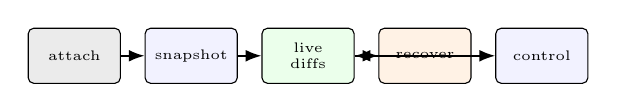
\begin{tikzpicture}[
  node distance=3mm,
  stage/.style={draw, rounded corners=2pt, align=center, font=\tiny,
    text width=11mm, minimum height=7mm, inner sep=1pt, fill=blue!5},
]
  \node[stage, fill=black!8] (attach) {attach};
  \node[stage, right=of attach] (snapshot) {snapshot};
  \node[stage, fill=green!8, right=of snapshot] (live) {live\\diffs};
  \node[stage, fill=orange!10, right=of live] (recover) {recover};
  \node[stage, right=of recover] (control) {control};
  \draw[flow] (attach) -- (snapshot);
  \draw[flow] (snapshot) -- (live);
  \draw[flow] (live) -- (recover);
  \draw[flow] (recover) -- (live);
  \draw[flow] (live) -- (control);
\end{tikzpicture}
\caption{Runtime lifecycle. A stream becomes useful after the first snapshot;
diffs are the normal path, while re-snapshot and subtree requests repair drift or
budgeted omissions.}
\label{fig:lifecycle}
\end{figure}

Figure~\ref{fig:arch} shows the end-to-end flow. Capture runs in the controlled
page, emits a snapshot and diffs through an injected transport, the relay fans
out raw frames under a one MiB cap, and the viewer reconstructs the page in an
inert iframe.

\begin{figure*}[t]
\centering
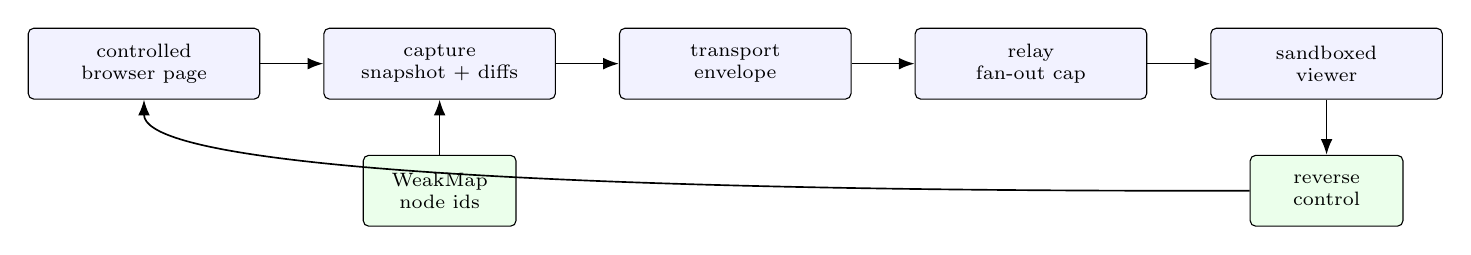
\begin{tikzpicture}[node distance=7mm and 8mm]
  \node[pswide] (page) {controlled\\browser page};
  \node[pswide, right=of page] (capture) {capture\\snapshot + diffs};
  \node[pswide, right=of capture] (transport) {transport\\envelope};
  \node[pswide, right=of transport] (relay) {relay\\fan-out cap};
  \node[pswide, right=of relay] (viewer) {sandboxed\\viewer};
  \node[psgreen, below=of capture] (identity) {WeakMap\\node ids};
  \node[psgreen, below=of viewer] (control) {reverse\\control};
  \draw[flow] (page) -- (capture);
  \draw[flow] (capture) -- (transport);
  \draw[flow] (transport) -- (relay);
  \draw[flow] (relay) -- (viewer);
  \draw[flow] (identity) -- (capture);
  \draw[flow] (viewer) -- (control);
  \draw[flow] (control.west) .. controls +(left:20mm) and +(down:12mm) .. (page.south);
\end{tikzpicture}
\caption{PhantomStream mirrors browser state rather than pixels. Capture emits
sanitized snapshot and diff frames addressed by stable node ids; the viewer
reconstructs the mirror in a sandbox and can map authorized input back to the
controlled page.}
\label{fig:arch}
\end{figure*}

\subsection{Snapshot and diff stream}

At stream start, capture clones the page body, walks the live and cloned trees in
parallel, and emits sanitized HTML plus sidecar metadata. Default mode inlines a
curated set of roughly 85 visual CSS properties. This is a production-driven
choice: full computed-style enumeration over hundreds of properties made heavy
pages unusably slow, while the curated list preserves common visual fidelity.
Opt-in CSSOM mode transports scoped stylesheet sources and live stylesheet ops
for hosts that prefer stylesheet-centric capture.

After the snapshot, a MutationObserver batches structural, attribute, and text
changes on requestAnimationFrame so delivery follows the page's paint cadence.
Diff ops are addressed by opaque node ids. Added subtrees carry their own
serialized HTML and preorder \code{nodeIds} sidecars so the renderer can index
new mirror nodes without selector lookup.

\subsection{Protocol frames and recovery}

The wire protocol is intentionally small. The dominant frame is the snapshot:
sanitized body HTML, viewport dimensions, scroll position, shell attributes,
sidecar node ids, open shadow-root payloads, accessible frame payloads, style
sources, and snapshot counters. Incremental mutation frames carry add, remove,
text, attribute, reorder, value, media, and frame-refresh operations. Independent
side channels carry scroll, overlay, dialog, media synchronization, media hints,
and subtree responses. Each frame includes enough stream identity for the
renderer to reject cross-generation updates once a fresh snapshot has replaced
the previous view.

Recovery is part of the normal protocol, not an exceptional control path. If a
snapshot would exceed the relay budget, capture drops whole offscreen subtrees
above a viewport-relative threshold and records placeholders with node ids. The
viewer can later request one of those subtrees when the user scrolls, focuses a
region, or asks the host to inspect a missing area. If the renderer detects that
diff application has drifted too far from its indexed tree, it latches a
re-snapshot request instead of continuing to apply diffs against uncertain
state. This keeps the renderer simple: every recovery path returns to the same
snapshot-plus-index invariant.

\subsection{Stable identity without page mutation}

The original FSB design stamped \code{data-fsb-nid} attributes onto the observed
page. The standalone package removes that mutation. Capture owns identity in a
\code{WeakMap<Element,string>} and emits ids only as wire sidecars. The renderer
builds a private \code{Map} from ids to mirror nodes after sanitization. This
keeps page-owned attributes ordinary page data and still lets overlays, subtree
requests, value diffs, media state, and remote control address the same node.

\subsection{Modern DOM and media}

The mirror handles several browser features that ordinary mutation streams miss.
Open shadow roots serialize as \code{shadowRoots[]} sidecars tied to host ids.
Same-origin iframes serialize as scoped \code{frames[]} payloads, while
cross-origin frames remain content-free placeholders. Form control values emit
property diffs because many value changes do not appear as DOM mutations.

Media is mirrored by reference. Image, video, and audio URLs travel as URL
strings and small playback-state messages; the relay never carries media bytes.
Progressive media uses a \code{STREAM.MEDIA} side channel and a pure drift
reconciler. Adaptive HLS or DASH can be driven from the parent realm through an
optional lazy player and manifest hints. Player code never runs inside the
sandboxed mirror iframe.

\subsection{Remote control contract}

Remote control is modeled as a separate protocol layered over the mirror. The
viewer can resolve a node id to a host-document rectangle, highlight it, and
return the active stream and snapshot identity associated with that rectangle.
It can also translate pointer coordinates through the scale-to-fit mapping of
the iframe. It does not directly mutate the controlled page. Instead, a host
adapter validates and normalizes control frames, applies an authorization state
machine, and dispatches browser-native actions only when control is active.

This separation is important for agent supervision. It means a passive viewer
can remain fully inert while still showing semantic targets. It also means the
same mirror can be embedded in different execution environments. A Playwright
host can dispatch through Playwright primitives, an extension host can dispatch
through content-script events, and a bookmarklet host can restrict itself to
local inspection. The protocol object that crosses the relay is a request, not
an implicit grant of authority.

% --- Reliability and Security --------------------------------------------
\section{Reliability and Security}

The production lesson behind PhantomStream is that a browser mirror fails in
small ways before it fails completely. A mutation queue can stall, a service
worker can be evicted, a page can exceed a relay cap, a start request can race
module load, and a late diff from a previous session can arrive after a new page
has loaded. The system makes these failure modes explicit. A content-side
watchdog force-flushes stale queues. An MV3 alarm watchdog can request a fresh
snapshot after service-worker eviction. Every stream frame carries session and
snapshot identity; stale frames are rejected. Snapshots are budgeted under the
relay cap by dropping whole offscreen subtrees after a single layout-read pass,
and dropped subtrees can be requested later by node id.

Security is a two-sided pipeline. Capture routes every serialization path through
a named \code{sanitizeForWire} chokepoint before transport. Render routes add-op
HTML, shadow roots, frame payloads, subtree responses, attributes, and CSSOM text
through render-side sanitizers before DOM insertion. The viewer document carries
a CSP meta policy and is hosted in an iframe whose sandbox token is exactly
\code{allow-same-origin}. The absence of \code{allow-scripts} is load bearing:
mirrored markup can render, but script in the mirror cannot execute.

Privacy masking is capture-side. Password values are always masked; hosts can
mask inputs, text regions, whole blocked subtrees, and asset or media URLs.
Because v2.0 mirrors assets by URL reference, signed CDN URLs and playback state
can themselves be private. The package therefore includes URL token stripping,
custom URL redaction, media selectors that omit URL and timeline state, a
fail-closed viewer fetch policy, and a document-level no-referrer posture.

\begin{table}[t]
\centering
\caption{Main runtime risks and current mitigations.}
\label{tab:threats}
\footnotesize
\begin{tabular}{@{}p{0.31\columnwidth} p{0.58\columnwidth}@{}}
\toprule
Risk & Mitigation \\
\midrule
Script execution in viewer & Render-side sanitizer, CSP, and an iframe sandbox
without \code{allow-scripts}. \\
Private content leakage & Capture-side masking for passwords, selectors, text,
assets, and media references. \\
Stale or crossed frames & Stream session and snapshot identity on live frames. \\
Relay budget exhaustion & One MiB relay cap, snapshot budget, offscreen subtree
truncation, and on-demand subtree recovery. \\
Unauthorized control & Host-owned authorization state plus normalized
remote-control messages. \\
\bottomrule
\end{tabular}
\end{table}

The relay is intentionally raw. It admits clients to rooms, classifies frame
sizes for diagnostics, enforces the per-message cap, and fans frames out without
understanding DOM semantics. This avoids making the relay a privileged parser for
untrusted page HTML. Endpoints own envelopes, compression, sanitization, and
authorization decisions. The tradeoff is that a malicious or buggy endpoint can
still send bad application payloads; the viewer must therefore retain its own
guards even when the relay has accepted a frame.

% --- Evaluation -----------------------------------------------------------
\section{Evaluation}

\subsection{Questions and methodology}

The benchmark asks three questions. First, how many bytes does each local mirror
representation produce. Second, how quickly does a post-action update become
observable. Third, what semantic information remains available to a receiver. The
benchmark is not a public-web study. It is a deterministic local corpus designed
to be rerun in the repository before the paper is rebuilt.

The corpus contains five pages: a static article, an infinite feed, a dashboard,
a modern-fidelity page with shadow DOM and a same-origin iframe, and a media page
with referenced video and audio. Each page runs three activities: idle, reading
and scrolling, and an agent-like mutation sequence. This produces
\PSBenchRunCount{} measured runs. The systems are PhantomStream, rrweb recorder
plus replay, and CDP \code{Page.startScreencast} PNG frames. The harness records
bytes, startup time, post-action latency, pixel-diff percentage against a final
page screenshot, and a semantic score. The semantic score is a four-point rubric:
DOM structure, incremental DOM changes, stable node identity, and reverse-control
targetability. PhantomStream scores four of four, rrweb scores two of four, and
CDP scores zero because it emits pixels only.

WebRTC screen capture is not claimed in this draft. Headless local Chromium does
not provide the same interactive \code{getDisplayMedia} permission surface as a
real user-driven capture session, so the harness records that baseline as
unavailable instead of substituting invented numbers.

\begin{figure}[t]
\centering
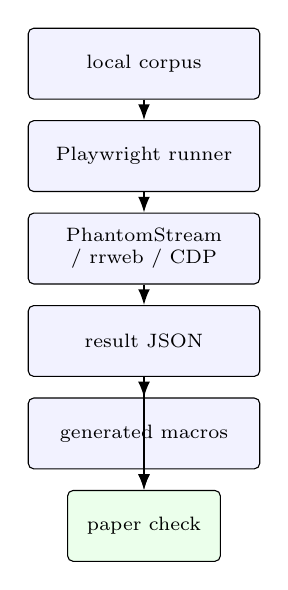
\begin{tikzpicture}[node distance=2.6mm]
  \node[pswide] (corpus) {local corpus};
  \node[pswide, below=of corpus] (runner) {Playwright runner};
  \node[pswide, below=of runner] (systems) {PhantomStream / rrweb / CDP};
  \node[pswide, below=of systems] (json) {result JSON};
  \node[pswide, below=of json] (tex) {generated macros};
  \node[psgreen, below=of tex] (paper) {paper check};
  \draw[flow] (corpus) -- (runner);
  \draw[flow] (runner) -- (systems);
  \draw[flow] (systems) -- (json);
  \draw[flow] (json) -- (tex);
  \draw[flow] (tex) -- (paper);
  \draw[flow] (json) -- (paper);
\end{tikzpicture}
\caption{Benchmark-to-paper pipeline. The paper imports generated result macros;
the validator fails if required metrics are missing, non-finite, or mismatched.}
\label{fig:benchpipe}
\end{figure}

\subsection{Harness implementation}

The benchmark harness starts a local HTTP server that serves only the deterministic
corpus, package source modules, and tiny local media placeholders. Each scenario
opens a fresh Playwright Chromium page at a fixed 1280 by 720 viewport. The
activity function runs inside the page and returns after deterministic scrolls,
input updates, or DOM insertions. The harness then waits a short settling window
and collects system-specific measurements.

PhantomStream is measured by injecting \code{createCapture} from the local source
tree and counting the UTF-8 bytes of every transport message. rrweb is measured
by injecting its browser bundle and counting serialized recorder events; the
harness also replays those events to obtain a final screenshot for the pixel-diff
metric. CDP is measured by enabling \code{Page.startScreencast} and summing the
decoded PNG frame bytes delivered by \code{screencastFrame} events. For all
systems, startup time is the delay to the first useful frame or event, and
post-action latency is the delay from the activity start timestamp to the first
subsequent update.

The output contract is deliberately strict. The JSON result file records the
environment, package version, corpus, activity list, baseline availability,
per-scenario metrics, summary medians, and project metrics. A generated TeX file
contains only macros derived from that JSON. The validator checks that all
expected systems produced results, WebRTC is explicitly marked unavailable, no
numeric metric is \code{NaN}, and the paper imports the generated macros rather
than copying numbers by hand.

\begin{table}[t]
\centering
\caption{Deterministic local benchmark corpus.}
\label{tab:corpus}
\footnotesize
\begin{tabular}{@{}l l p{0.38\columnwidth}@{}}
\toprule
Page & Activities & Purpose \\
\midrule
article & idle, reading, agent & static text and scroll pressure \\
feed & idle, reading, agent & appended cards and list growth \\
dashboard & idle, reading, agent & tables, cards, and input changes \\
fidelity & idle, reading, agent & shadow DOM, iframe, forms \\
media & idle, reading, agent & referenced video and audio URLs \\
\bottomrule
\end{tabular}
\end{table}

\subsection{Bytes and latency}

Figure~\ref{fig:bytes} reports median bytes per run. PhantomStream's median was
\PSPhantomMedianKB{} KB. CDP screencast's median was \PSCDPMedianKB{} KB, so
PhantomStream used \PSReductionVsCDP{} percent fewer bytes in this local corpus.
rrweb's median was only \PSRrwebMedianKB{} KB, substantially smaller than
PhantomStream. This is the clearest tradeoff in the data. PhantomStream's
snapshot carries inline style and live-control metadata; rrweb's recorder emits a
more compact replay log.

\begin{figure}[t]
\centering
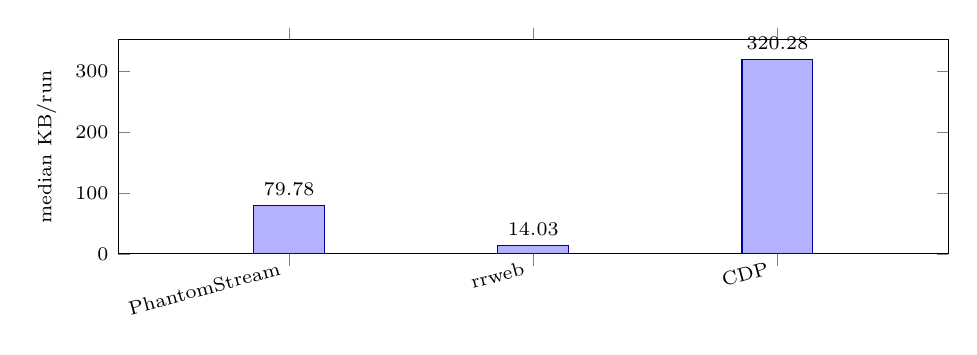
\begin{tikzpicture}
\begin{axis}[
  ybar,
  width=\columnwidth, height=43mm,
  bar width=9mm,
  ymin=0,
  ylabel={median KB/run},
  symbolic x coords={PhantomStream,rrweb,CDP},
  xtick=data,
  nodes near coords,
  every node near coord/.append style={font=\scriptsize},
  xticklabel style={font=\scriptsize, rotate=15, anchor=east},
  yticklabel style={font=\scriptsize},
  ylabel style={font=\scriptsize},
  enlarge x limits=0.35,
]
\addplot[draw=blue!60!black, fill=blue!30] coordinates
  {(PhantomStream,\PSPhantomMedianKB) (rrweb,\PSRrwebMedianKB) (CDP,\PSCDPMedianKB)};
\end{axis}
\end{tikzpicture}
\caption{Median bytes per deterministic local run. PhantomStream is smaller than
CDP screencast but larger than rrweb's compact recorder stream.}
\label{fig:bytes}
\end{figure}

Figure~\ref{fig:latency} reports median post-action latency over non-idle
activities. PhantomStream's median was \PSPhantomLatencyMs{} ms, close to rrweb's
\PSRrwebLatencyMs{} ms and below CDP's \PSCDPLatencyMs{} ms. These numbers are
local headless measurements, not WAN latency claims. They do show that the DOM
stream can react in the same order of magnitude as a recorder and earlier than
the first post-action screencast frame in this setup.

\begin{figure}[t]
\centering
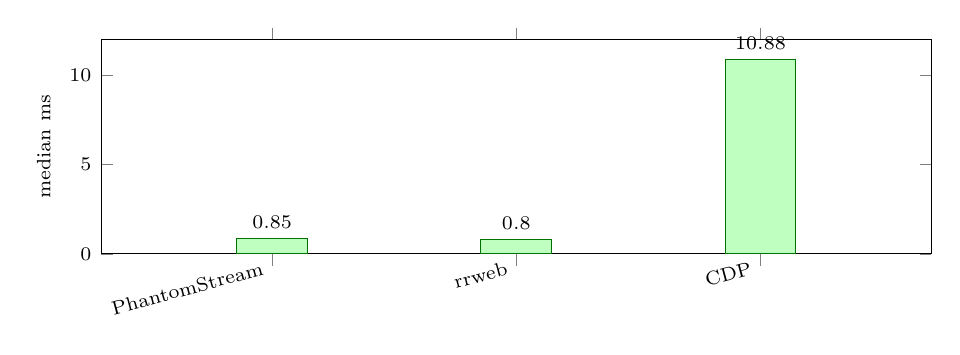
\begin{tikzpicture}
\begin{axis}[
  ybar,
  width=\columnwidth, height=43mm,
  bar width=9mm,
  ymin=0,
  ylabel={median ms},
  symbolic x coords={PhantomStream,rrweb,CDP},
  xtick=data,
  nodes near coords,
  every node near coord/.append style={font=\scriptsize},
  xticklabel style={font=\scriptsize, rotate=15, anchor=east},
  yticklabel style={font=\scriptsize},
  ylabel style={font=\scriptsize},
  enlarge x limits=0.35,
]
\addplot[draw=green!45!black, fill=green!25] coordinates
  {(PhantomStream,\PSPhantomLatencyMs) (rrweb,\PSRrwebLatencyMs) (CDP,\PSCDPLatencyMs)};
\end{axis}
\end{tikzpicture}
\caption{Median post-action latency on non-idle local activities.}
\label{fig:latency}
\end{figure}

\subsection{Fidelity and semantics}

The pixel-diff result is intentionally simple. CDP frames and PhantomStream final
snapshots both reached a median 0 percent pixel-diff against the final page
screenshot in this local corpus. rrweb replay had a median \PSRrwebVisualDiff{}
percent pixel-diff, mostly from replay viewport and timing differences in the
headless harness. The semantic score separates the systems more sharply:
PhantomStream preserves all four rubric dimensions, rrweb preserves DOM
structure and incremental change but not public live targetability, and CDP
preserves none.

\begin{table}[t]
\centering
\caption{Median local fidelity and semantic scores.}
\label{tab:fidelity}
\footnotesize
\begin{tabular}{@{}l c c@{}}
\toprule
System & pixel diff (\%) & semantic score \\
\midrule
PhantomStream & \PSPhantomVisualDiff & \PSPhantomSemantic \\
rrweb & \PSRrwebVisualDiff & \PSRrwebSemantic \\
CDP screencast & \PSCDPVisualDiff & \PSCDPSemantic \\
\bottomrule
\end{tabular}
\end{table}

\begin{figure}[t]
\centering
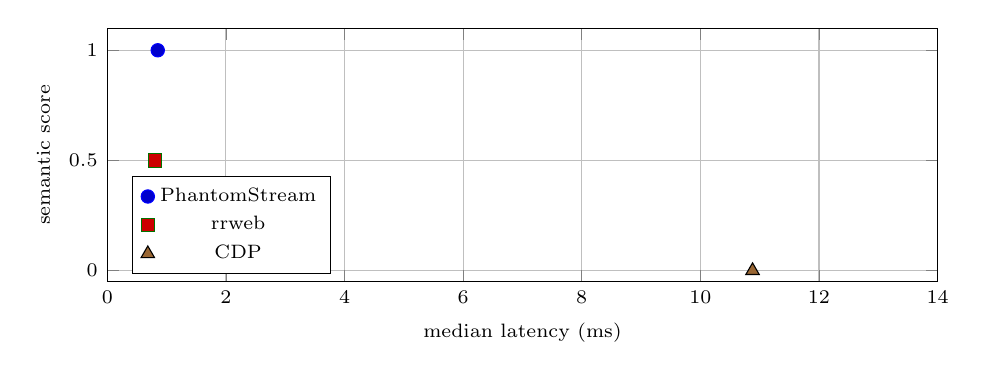
\begin{tikzpicture}
\begin{axis}[
  width=\columnwidth, height=48mm,
  xmin=0, xmax=14,
  ymin=-0.05, ymax=1.1,
  xlabel={median latency (ms)},
  ylabel={semantic score},
  xlabel style={font=\scriptsize},
  ylabel style={font=\scriptsize},
  xticklabel style={font=\scriptsize},
  yticklabel style={font=\scriptsize},
  grid=both,
  legend style={font=\scriptsize, at={(0.03,0.03)}, anchor=south west},
]
\addplot+[only marks, mark=*, mark size=2.4pt, blue] coordinates {(\PSPhantomLatencyMs,\PSPhantomSemantic)};
\addlegendentry{PhantomStream}
\addplot+[only marks, mark=square*, mark size=2.4pt, green!45!black] coordinates {(\PSRrwebLatencyMs,\PSRrwebSemantic)};
\addlegendentry{rrweb}
\addplot+[only marks, mark=triangle*, mark size=2.8pt, black] coordinates {(\PSCDPLatencyMs,\PSCDPSemantic)};
\addlegendentry{CDP}
\end{axis}
\end{tikzpicture}
\caption{Latency and semantic addressability tradeoff in the local benchmark.
Lower-left is fast but less actionable; upper-left is the supervision target.}
\label{fig:tradeoff}
\end{figure}

\subsection{Implementation and assurance}

PhantomStream version \PSPackageVersion{} is a source-first ESM package with one
runtime dependency, \code{ws}. The implementation-facing JavaScript surface in
\code{src}, \code{bin}, and \code{examples} contains \PSProdFiles{} files and
about \PSProdLoc{} lines. The test suite currently passes \PSTestCount{} tests
across \PSTestFiles{} test files. The most important tests are not only unit
tests; they include a differential oracle that runs reference and extracted
captures over frozen fixtures, checks all intentional divergences against a
ledger, and fails loudly on undeclared drift.

The benchmark is not yet in the same category as the test suite. It is a draft
research harness whose purpose is to prevent the paper from making unsupported
claims. Its scenarios are small enough to run during manuscript work and varied
enough to catch obvious regressions in snapshot size, diff flow, replay fidelity,
and baseline availability. That is the right role for this draft: it turns the
paper's charts into reproducible artifacts before the project invests in a much
larger public corpus.

% --- Discussion -----------------------------------------------------------
\section{Discussion}

The benchmark makes PhantomStream's position clearer than the original outline
did. Against CDP screencast, the DOM-native mirror has the expected bandwidth and
latency advantage in local runs while preserving semantic control handles. Against
rrweb, PhantomStream is not the byte winner. That is acceptable because the
systems optimize different products. rrweb is a compact session recorder.
PhantomStream is a live, sandboxed, remotely controllable mirror. It spends bytes
on inline visual state, stable ids, side channels, and viewer safety.

This distinction matters for browser agents. An agent-observability surface needs
to answer questions that a replay log or a frame stream does not answer by
default: which element is highlighted, whether a remote click can be mapped back
through the mirror, whether a late diff belongs to the current tab, whether a
masked subtree leaked, and whether a viewer fetch is allowed. PhantomStream makes
those concerns explicit protocol and security decisions.

Pixels still have a place. They are the right fallback for WebGL, DRM video,
native browser UI, and other surfaces that intentionally do not expose useful DOM
state. They also provide a human-verifiable last resort when a DOM mirror is
wrong. PhantomStream should therefore be understood as the primary channel for
structured web content, not as a claim that every browser pixel should be
serialized as DOM. A robust agent console will likely combine DOM-native
mirroring with selective pixel fallbacks for opaque regions.

The rrweb comparison is similarly nuanced. rrweb's compactness is a real result,
not an artifact to explain away. If the product is offline replay, rrweb's
representation is attractive. If the product is live supervision with targetable
nodes, explicit authority boundaries, and viewer fetch controls, a larger
message stream can be justified. The next paper revision should quantify this
boundary with ablations: no inline style, CSSOM-only style, no side channels, and
no control metadata.

% --- Limitations ----------------------------------------------------------
\section{Limitations}

This draft has three important limitations. First, the evaluation is local and
deterministic. It is suitable for regression and for an honest first paper draft,
but it is not yet a public-site study. The next corpus should use HAR
record/replay over real sites and should run each baseline under identical
network and browser conditions.

Second, WebRTC is not measured here. The browser API is permission mediated and
interactive by design \cite{screencapture}; a headless-only substitute would be a
weak claim. A later evaluation should run WebRTC from a real capture surface and
report its encoder settings.

Third, PhantomStream does not mirror everything. Cross-origin iframe content,
DRM/EME video, MSE media with no discoverable manifest, WebGL/canvas frame
streams, Web Audio, and mobile/non-Chromium contexts remain outside the current
contract or degrade to placeholders. These are mostly browser security and
bandwidth boundaries, not accidental omissions.

% --- Future Work ----------------------------------------------------------
\section{Future Work}

The next step is a full v2.1 evaluation harness: public HAR record/replay corpus,
scripted activity levels, WebRTC and CDP pixel baselines, rrweb live-mode replay,
style-capture ablations, and a failure taxonomy that combines perceptual and DOM
semantic metrics. The paper should also grow a primary-source related-work pass
on co-browsing systems, session replay, remote display protocols, and
agent-observability viewers. On the system side, useful extensions include a
cursor channel, opt-in budgeted canvas refresh, caret and selection mirroring,
and an rrweb-format export bridge for storage interoperability.

% --- Conclusion -----------------------------------------------------------
\section{Conclusion}

PhantomStream is a DOM-native live mirror for supervising browser agents. It
streams a sanitized snapshot and small node-addressed diffs, reconstructs the
page in a scriptless sandbox, preserves stable semantic handles, and supports
authorized reverse control. The current package is public, tested by
\PSTestCount{} automated tests, and measured by a deterministic local benchmark.
The results show the intended tradeoff: PhantomStream is far smaller than local
CDP screencast and keeps full semantic addressability, but it is larger than
rrweb's compact recorder stream. That is the core argument. Agent supervision
does not need only pixels, and it does not need only replay. It needs a live,
safe, semantically addressable mirror of the browser the agent controls.

% --- References -----------------------------------------------------------
\bibliographystyle{IEEEtran}
\bibliography{refs}

\end{document}
